% \documentclass[mat2, tisk]{fmfdelo}
% \documentclass[fin2, tisk]{fmfdelo}
\documentclass[isrm2, tisk]{fmfdelo}
% \documentclass[ped, tisk]{fmfdelo}
% Če pobrišete možnost tisk, bodo povezave obarvane,
% na začetku pa ne bo praznih strani po naslovu, …

%%%%%%%%%%%%%%%%%%%%%%%%%%%%%%%%%%%%%%%%%%%%%%%%%%%%%%%%%%%%%%%%%%%%%%%%%%%%%%%
% METAPODATKI
%%%%%%%%%%%%%%%%%%%%%%%%%%%%%%%%%%%%%%%%%%%%%%%%%%%%%%%%%%%%%%%%%%%%%%%%%%%%%%%

% - vaše ime
\avtor{Tim Kalan}

% - naslov dela v slovenščini
\naslov{Skupinsko generirani podpisi}

% - naslov dela v angleščini
\title{Multisignatures}

% - ime mentorja/mentorice s polnim nazivom:
%   - doc.~dr.~Ime Priimek
%   - izr.~prof.~dr.~Ime Priimek
%   - prof.~dr.~Ime Priimek
%   za druge variante uporabite ustrezne ukaze
\mentor{doc.~dr.~Tilen Marc}
% \somentor{...}
% \mentorica{...}
% \somentorica{...}
% \mentorja{...}{...}
% \somentorja{...}{...}
% \mentorici{...}{...}
% \somentorici{...}{...}

% - leto magisterija
\letnica{2024}

% - povzetek v slovenščini
%   V povzetku na kratko opišite vsebinske rezultate dela. Sem ne sodi razlaga
%   organizacije dela, torej v katerem razdelku je kaj, pač pa le opis vsebine.
\povzetek{Tukaj napišemo povzetek vsebine. Sem sodi razlaga vsebine in ne opis tega, kako je delo organizirano.}

% - povzetek v angleščini
\abstract{An abstract of the work is written here. This includes a short description of
the content and not the structure of your work.}

% - klasifikacijske oznake, ločene z vejicami
%   Oznake, ki opisujejo področje dela, so dostopne na strani https://www.ams.org/msc/
\klasifikacija{94A60, 11T71}

% - ključne besede, ki nastopajo v delu, ločene s \sep
\kljucnebesede{digitalni podpis\sep kriptografija}

% - angleški prevod ključnih besed
\keywords{digital signature\sep cryptography} % angleški prevod ključnih besed

% - neobvezna zahvala
\zahvala{
  Neobvezno.
  Zahvaljujem se \dots
}

% - program dela, ki ga napiše mentor z osnovno literaturo
\programdela{
  Mentor naj napiše program dela skupaj z osnovno literaturo.
}

\osnovnaliteratura{
% Literatura mora biti tukaj posebej samostojno navedena (po pomembnosti) in ne
% le citirana. V tem razdelku literature ne oštevilčimo po svoje, ampak uporabljamo
% ukaz \vnosliterature, v katerega vpišemo citat
  \vnosliterature{micali2001asm}
  % \vnosliterature{gurtin1982introduction}
  % \vnosliterature{zienkiewicz2000finite}
  % \vnosliterature{STtemplate}
}

% - ime datoteke z viri (vključno s končnico .bib), če uporabljate BibTeX
\literatura{literatura.bib}

%%%%%%%%%%%%%%%%%%%%%%%%%%%%%%%%%%%%%%%%%%%%%%%%%%%%%%%%%%%%%%%%%%%%%%%%%%%%%%%
% DODATNE DEFINICIJE
%%%%%%%%%%%%%%%%%%%%%%%%%%%%%%%%%%%%%%%%%%%%%%%%%%%%%%%%%%%%%%%%%%%%%%%%%%%%%%%

% naložite dodatne pakete, ki jih potrebujete
\usepackage{units}        % fizikalne enote kot \unit[12]{kg} s polovico nedeljivega presledka, glej primer v kodi
\usepackage{graphicx}     % za slike
% \usepackage{tikz}
% VEČ ZANIMIVIH PAKETOV
% \usepackage{array}      % več možnosti za tabele
% \usepackage[list=true,listformat=simple]{subcaption}  % več kot ena slika na figure, omogoči slika 1a, slika 1b
% \usepackage[all]{xy}    % diagrami
% \usepackage{doi}        % za clickable DOI entrye v bibliografiji
% \usepackage{enumerate}     % več možnosti za sezname

% Za barvanje source kode
% \usepackage{minted}
% \renewcommand\listingscaption{Program}

% Za pisanje psevdokode
% \usepackage{algpseudocode}  % za psevdokodo
% \usepackage{algorithm}
% \floatname{algorithm}{Algoritem}
% \renewcommand{\listalgorithmname}{Kazalo algoritmov}

% deklarirajte vse matematične operatorje, da jih bo LaTeX pravilno stavil
% \DeclareMathOperator{\...}{...}

% vstavite svoje definicije ...
\newcommand{\R}{\mathbb R}
\newcommand{\N}{\mathbb N}
\newcommand{\Z}{\mathbb Z}
% Lahko se zgodi, da je ukaz \C definiral že paket hyperref,
% zato dobite napako: Command \C already defined.
% V tem primeru namesto ukaza \newcommand uporabite \renewcommand
\newcommand{\C}{\mathbb C}
\newcommand{\Q}{\mathbb Q}

%%%%%%%%%%%%%%%%%%%%%%%%%%%%%%%%%%%%%%%%%%%%%%%%%%%%%%%%%%%%%%%%%%%%%%%%%%%%%%%
% ZAČETEK VSEBINE
%%%%%%%%%%%%%%%%%%%%%%%%%%%%%%%%%%%%%%%%%%%%%%%%%%%%%%%%%%%%%%%%%%%%%%%%%%%%%%%

\begin{document}

\section{Uvod}
% Napišite kratek zgodovinski in matematični uvod.  Pojasnite motivacijo za problem, kje
% nastopa, kje vse je bil obravnavan. Na koncu opišite tudi organizacijo dela -- kaj je v
% katerem razdelku.
Odkar se je na svetu pojavil koncept (ročnega) podpisa, je večina primerov uporabe temeljila na
pridobivanju podpisov več deležnikov. Odličen primer je npr.\ Deklaracija neodvisnosti Združenih 
držav Amerike. SLIKA?. 

V prejšnjem stoletju je vzpon računalnika in napredek v kriptografiji privedel do \textit{digitalnih
podpisov}. Ti odlično nadomeščajo ročni podpis, prav tako omogočajo, da se skupina podpiše tako, 
da vsak član poda svoj podpis. Vendar tu lahko z malo matematike poskrbimo, da se skupina lahko 
podpiše tako, da vsi člani skupaj oddajo en sam podpis, ki priča o podpisu celotne skupine. Tako 
razbremenimo preverjalca podpisov, kar je ključno v sistemih, kjer je računska moč omejena ali 
pa draga (npr.\ pri tehnologiji veriženja blokov).

\section{Kriptografske osnove}
Preden si lahko pogledamo točno kako lahko skupina generira en sam podpis besedila, si moramo 
pogledati nekaj kriptografskih osnov. Bolj komplicirane stvari bodo opisane sproti, ideja tega 
poglavja je predstaviti stvari, ki so predpogoj za branje kakršnegakoli kriptografskega 
besedila.

\subsection{Zgoščevalne funkcije}
V grobem so (kriptografske) \textit{zgoščevalne funkcije} funkcije, ki prejmejo poljubno dolg binarni 
niz (ki lahko predstalja besede, številke, celotne dokumente, \dots), vrnejo pa binarni niz, ki ima 
vnaprej določeno dolžino. Tem rezultatom pravimo \textit{zgostitve}. V grobem si od zgoščevalnih 
funkcij želimo naslednje lastnosti:
\begin{itemize}
    \item \textbf{Določenost} pomeni, da bo zgoščevanje enakih nizov vedno privedlo do enakega 
        odgovora. 
    \item \textbf{Učinkovitost} pomeni, da lahko računalnih izračuna poljubno zgostitev v doglednem 
        času.
    \item \textbf{Enosmernost} pomeni, da iz predložene zgostitve zelo težko ugotovimo, kater niz 
        je funkcija prejela kot vhod.
    \item \textbf{Skoraj brez trčenj} pomeni, da je verjetnost, da imata dva izraza enako zgostitev,
        majhna. Želimo tudi, da je zelo težko najti dva niza z enako zgostitvijo.
\end{itemize}

\begin{primer}
    Ena izmed najbolj znanih zgostitvenih funkcij je \texttt{SHA-256}. Njeno ime pomeni \textit{Secure 
    Hashing Algorithm} (slov.\ varen zgostitveni algoritem), $256$ pa predstavlja dolžino zgostitve. 
    Pogostokrat to ime zasledimo pri nameščanju programske opreme, služi kot avtentikator, da smo res 
    naložili pravo stvar.

    Za primer si lahko ogledamo zgostitvi dveh podobnih nizov, \textit{Ljubljana} in \textit{Ljubljena}. 
    Kljub podobnosti bomo videli, da sta rezultata popolnoma drugačna, kar si tudi želimo pri zgostitvenih 
    funkcijah.
    \begin{verbatim}
    SHA-256(Ljubljana) =
    b7f147d8b4a6703a951336654355071f9752385f85d0860379e99b484aee7a82

    SHA-256(Ljubljena) =
    995d2d8ffb40e1838219e65dd2c665701ba34a90e11f7195a4b791838b6787fe
    \end{verbatim}
    Za preglednost nismo prevajali besed v binarne nize, to bi storili npr.\ z \texttt{ASCII} ali \texttt{UTF-8}
    tabelo. Prav tako smo rezultat napisali v šestnajstiškem sistemu, saj je tako krajši.
\end{primer}

\subsubsection{Model slučajnega oraklja}

\subsection{Kriptografija javnega ključa}
Prve šifre, ki smo jih uporabljaji ljudje, so bile \textit{simetrične}, kar pomeni, da sta osebi 
za komunikacijo obe morali poznati skriven \textit{ključ}, ki je definiral, kako je bila šifra 
ustvarjena. 

\begin{primer}[Cezarjeva šifra]
    Ena najbolj znanih šifer, ki izvira iz Antičnega Rima, je \textit{Cezrjeva šifra}. Njen ključ 
    je število, ki je krajše od dolžine naše abecede, v Cezarjevem primeru je bilo to število $3$.
    Šifra potem deluje tako, da vsako črko zamaknemo za toliko mest v abecedi, kolikor definira 
    ključ. Npr.\ za slovensko abecedo, bi šifra zamaknila črke:
    \begin{verbatim}
        A B C Č D E F G H I J K L M N O P R S Š T U V Z Ž
        Č D E F G H I J K L M N O P R S Š T U V Z Ž A B C
    \end{verbatim}
    To bi izraz \texttt{JAVNI KLJUČ} preslikalo v \texttt{MČARL NOMŽF}. Cezarjeva šifra se imenuje 
    tudi \textit{zamična šifra}.
\end{primer}

V prejšnjem stoletju pa se je pojavila alternativa, imenovana \textit{asimetrična kriptografija}, oz.\
\textit{kriptografija javnega ključa}. Glavna prednost te je, da osebi za komunikacijo ne rabita 
poznati enakega skrivnega ključa, vendar ima vsak od njiju par ključev, ki ju imenujemo \textit{javni 
ključ} (angl.\ \textit{public key}) in \textit{zasebni ključ} (angl.\ \textit{secret/private key})in 
označimo kot par $(\text{pk}, \text{sk})$. Vsaka oseba objavi svoj javni ključ in poskrbi, da nihče 
ne izve, kaj je njen zasebni ključ. 

Šifriranje potem poteka tako, da pridobimo javni ključ od osebe, s katero želi komunicirati, ga uporabi
za šifriranje in objavi šifrirano sporočilo. Lastnik ustreznega zasebnega ključa (vsakemu javnemu pripada 
natanko en zasebni) potem pridobi šifrirano sporočilo in ga z zasebnim ključem odšifrira. Kriptosistemi 
delujejo na način, da lahko sporočilo, šifrirano z javnim ključem odšifrira samo ustrezen zasebni ključ. 
Tako zagotovimo varno komunikacijo. 

\begin{primer}[RSA]
    En prvih algoritmov javnega ključa, ki se uporablja še danes, je \textit{RSA}. Njegova varnost izhaja 
    iz (domnevne) težavnosti problema iskanja prafaktorjev. Svoj ključ definiramo tako, da si izberemo dve 
    (zelo veliki) praštevili $p$ in $q$, ter ju zmnožimo v $n = pq$. Za primer vzemimo $p = 23$ in 
    $q = 17$. $n$ je potem enak $391$. Izbrati si moramo še eksponent $e$, vzemimo npr. $e = 3$. Naš 
    javni ključ je potem par 
    $$ 
    (n, e) = (391, 3).
    $$
    Postopek šifriranja poteka tako, da oseba, s katero komuniciramo, izbere sporočilo $m$, npr.\ 
    $m = 10$, pridobi naš javni ključ, in izračuna šifro $c$ kot
    $$   
    c = m^e \bmod{n} = 10^3 \bmod{n} = 218.
    $$
    Dogovoriti se moramo še o zasebnem ključu. Za to bomo potrebovali eksponent za odšifriranje $d$,
    tako da bo veljalo 
    $$
    (m^e)^d \equiv 1 \pmod{\varphi(n)},
    $$ 
    kjer $\varphi$ označuje Eulerjevo funkcijo fi. Iščemo torej multiplikativni inverz eksponenta 
    $e$, modulo $\varphi(n)$. V našem primeru je to $d = 235$. Zasebni ključ je potem 
    $$ 
    (p, q, d) = (23, 17, 235). 
    $$
    Iz zasebnega ključa torej lahko kadarkoli izračunamo javnega, saj enostavno zmnožimo $p$ in $q$ 
    ter izračunamo inverz, v splošnem pa iz $n$ učinkovito ne moremo pridobiti faktorjev $p$ in $q$,
    kar nam daje varnost.

    Ko prejmemo šifrirano sporočilo $c$, ga odšifriramo tako, da izračunamo
    $$
    m = c^d \bmod{n} = 218^{235} \bmod{391} = 10.   
    $$
\end{primer}

Poleg šifriranja, brez da bi si delili ključ, pa je kriptografija javnega ključa omogočila tudi 
\textit{digitalne podpise}. Ti so uporabljeni vsakič, ko pošljemo e-pošto ali dostopamo do katerekoli 
spletne strani. Delujejo na podoben način, kot šifriranje z javnim ključem, le da najprej uporabimo 
zasebni ključ na sporočilu, prek javnega ključa pa preverjamo veljavnost podpisa. Ponavadi sta šifrianje 
in podisovanje uporabljena hkrati, saj tako pošljemo šifrirano sporočilo, za katerega lahko oseba, 
s katero komuniciramo preveri, da je res prišlo od nas.

\subsection{Digitalni podpisi}
Ideja \textit{kriptografskih} ali \textit{digitalnih} podpisov je, da služijo kot izboljšava človeškega 
ročnega podpisa. Za razliko od ročnega podpisa, lahko z digitalnim dosežemo pravo identifikacijo 
posameznika, ki temelji na njegovem zasebnem ključu. Tako smo lahko za digitalno podpisan dokument 
prepričani, da ga je res podpisal lastnik točno določenega zasebnega ključa. 

Podpis dokumenta poteka nekoliko drugače, kot pri ročnih podpisih. Pri ročnem podpisu ta postane del 
dokumenta, digitalni podpis pa je od njega ločen, vseeno pa nastane s pomočjo zgostitve podpisanega 
dokumenta, zato bo podpis za dva različna dokumenta vedno drugačen.

Ostane še vprašanje preverjanja avtentičnosti podpisa. Pri ročnem podpisu to lahko storimo prek 
primerjave z znanim, preverjeno avtentičnim podpisom. Ta postopek je zamuden in nenatančen, veliko 
večino ročnih podpisov je moč ponarediti z nekaj prakse. Preverjanje digitalnega podpisa pa temelji 
na kriptografiji javnega ključa. Ker je podpis nastal s pomočjo podpisnikovega zasebnega ključa,
lahko s pomočjo ujemajočega javnega ključa preverimo avtentičnost.

\begin{definicija}
    \textbf{Digitalni} ali \textbf{kriptografski podpis} $\mathcal{S} = (G, S, V)$ je trojica 
    učinkovitih algoritmov $G$ za ustvarjanje ključa, $S$ za podpisovanje in $V$ za preverjanje 
    podpisa. Definirana je nad končno množico možnih sporočil $\mathcal{M}$, vrnjeni podpis pa 
    leži v v končni množici podpisov $\Sigma$.
    \begin{itemize}
        \item $G$ je naključnostni algoritem za ustvarjanje para ključev $(\text{pk}, \text{sk})$, 
            ki ne prejme nobenega argumenta. $\text{pk}$ je javni kljč za preverjanje avtentičnosti 
            podpisa, $\text{sk}$ pa je zasebni ključ za podpisovanje. 
        \item $S$ je naključnostni algoritem, ki za svoja argumenta prejme zasebni ključ $\text{sk}$ 
            in sporočilo $m$, vrne pa podpis $\sigma$ spročila $m$ z zasebnim ključem $\text{sk}$ 
            oz.\ 
            $$ 
            \sigma = S(\text{sk}, m).
            $$
        \item $V$ je determinističen algoritem, ki preverja veljavnost podpisov. Za svoje arugmente 
            prejme javni ključ $\text{pk}$, sporočilo $m$ in podpis $\sigma$, vrne $veljaven$, če je podpis 
            veljaven in $neveljaven$, sicer. Velja torej
            $$ 
            V(\text{pk}, m, \sigma) = 
            \begin{cases}
                veljaven, & \sigma = S(\text{sk}, m), \\
                neveljaven, & \sigma \neq S(\text{sk}, m).
            \end{cases}
            $$
    \end{itemize}
\end{definicija}

\subsubsection{Ustvarjanje ključa}
\subsubsection{Podpisovanje}
\subsubsection{Preverjanje podpisa}

\subsubsection{Primer: Schnorrov podpis}

\subsection{Drugo}
Merklova drevesa, dokazi brez razkritja znanja, slučajni oraklji, fiat-shamirjeva hevristika,

\section{Matematično ozadje}
\subsection{Modularna aritmetika}
kongruence, modulo,

\subsection{Multiplikativne grupe modulo $n$}
multiplikativni inverz, red elementa, diskretni logaritem

\section{Pregled skupinskih podpisov}

\section{Skupinsko generirani podpisi na podlagi Schnorrovega podpisa}
Povzeto po~\cite{micali2001asm}.

\section{Skupinsko generirani podpisi v splošnem}

% \section{Integrali po \texorpdfstring{$\omega$}{ω}-kompleksih}
% \subsection{Definicija}
% \begin{definicija}
%   Neskončno zaporedje kompleksnih števil, označeno z $\omega = (\omega_1, \omega_2, \ldots)$,
%   se imenuje \emph{$\omega$-kompleks}.\footnote{To ime je izmišljeno.}
%
%   Črni blok zgoraj je tam namenoma. Označuje, da \LaTeX{} ni znal vrstice prelomiti pravilno
%   in vas na to opozarja. Preoblikujte stavek ali mu pomagajte deliti problematično besedo z
%   ukazom \verb|\hyphenation{an-ti-ko-mu-ta-ti-ven}| v preambuli.
% \end{definicija}
% \begin{trditev}[Znano ime ali avtor]
%   \label{trd:obstoj-omega}
%   Obstaja vsaj en $\omega$-kompleks.
% \end{trditev}
% \begin{proof}
%   Naštejmo nekaj primerov:
%   \begin{align}
%     \omega &= (0, 0, 0, \dots), \label{eq:zero-kompleks} \\
%     \omega &= (1, i, -1, -i, 1, \ldots), \nonumber \\
%     \omega &= (0, 1, 2, 3, \ldots). \nonumber \qedhere  % postavi QED na zadnjo vrstico enačbe
%   \end{align}
% \end{proof}
%
% \section{Tehnični napotki za pisanje}
%
% \subsection{Sklicevanje in citiranje}
% Za sklice uporabljamo \verb|\ref|, za sklice na enačbe \verb|\eqref|, za citate \verb|\cite|. Pri
% sklicevanju in citiranju sklicano številko povežemo s prejšnjo besedo z nedeljivim presledkom
% $\sim$, kot npr.\ \verb|iz trditve~\ref{trd:obstoj-omega} vidimo|.
%
% \begin{primer}
%   Zaporedje~\eqref{eq:zero-kompleks} iz dokaza trditve~\ref{trd:obstoj-omega} na
%   strani~\pageref{trd:obstoj-omega} lahko najdemo tudi v Spletni enciklopediji zaporedij~\cite{oeis}.
%   Citiramo lahko tudi bolj natančno~\cite[trditev 2.1, str.\ 23]{lebedev2009introduction}.
% \end{primer}
%
% \subsection{Okrajšave}
% Pri uporabi okrajšav \LaTeX{} za piko vstavi predolg presledek, kot npr. tukaj. Zato se za vsako
% piko, ki ni konec stavka doda presledek običajne širine z ukazom \verb*|\ |, kot npr.\ tukaj.
% Primerjaj z okrajšavo zgoraj za razliko.
%
% \subsection{Vstavljanje slik}
% Sliko vstavimo v plavajočem okolju \texttt{figure}. Plavajoča okolja \emph{plavajo} po tekstu, in
% jih lahko postavimo na vrh strani z opcijskim parametrom `\texttt{t}', na lokacijo, kjer je v kodi s
% `\texttt{h}', in če to ne deluje, potem pa lahko rečete \LaTeX u, da ga \emph{res} želite tukaj,
% kjer ste napisali, s `\texttt{h!}'. Lepo je da so vstavljene slike vektorske (recimo \texttt{.pdf}
% ali \texttt{.eps} ali \texttt{.svg}) ali pa \texttt{.png} visoke resolucije (več kot
% \unit[300]{dpi}).  Pod vsako sliko je napis in na vsako sliko se skličemo v besedilu. Primer
% vektorske slike je na sliki~\ref{fig:sample}. Vektorsko sliko prepoznate tako, da močno
% zoomate v sliko, in še vedno ostane gladka. Več informacij je na voljo na
% \url{https://en.wikibooks.org/wiki/LaTeX/Floats,_Figures_and_Captions}. Če so slike bitne, kot na
% primer slika~\ref{fig:image}, poskrbite, da so v dovolj visoki resoluciji.
%
% \begin{figure}[h]
%   \centering
%   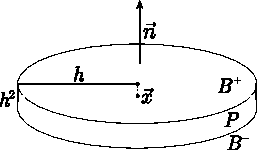
\includegraphics[width=0.6\textwidth]{images/sample.pdf}
% % \caption[caption za v kazalo]{Dolg caption pod sliko}
%   \caption[Primer vektorske slike.]{Primer vektorske slike z oznakami v enaki pisavi, kot jo
%      uporablja \LaTeX{}.  Narejena je s programom Inkscape, \LaTeX{} oznake so importane v
%      Inkscape iz pomožnega PDF.}
%   \label{fig:sample}
% \end{figure}
%
% \begin{figure}[h]
%   \centering
%   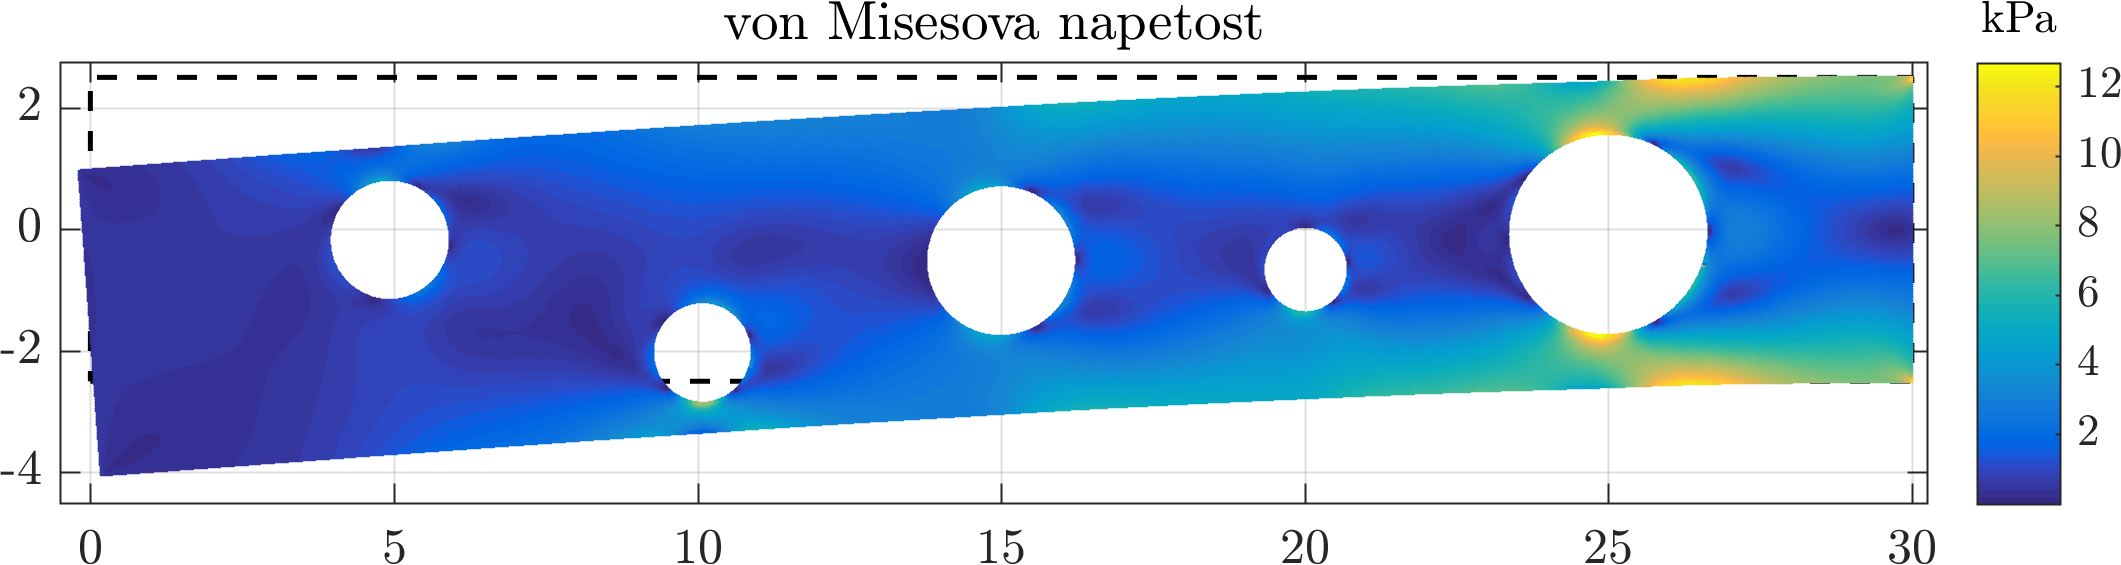
\includegraphics[width=0.8\textwidth]{images/image.png}
%   \caption[Primer bitne slike.]{Primer bitne slike, izvožene iz Matlaba. Poskrbite, da so slike v
%   dovolj visoki resoluciji in da ne vsebujejo prosojnih elementov (to zahteva PDF/A-1b format).}
%   \label{fig:image}
% \end{figure}
%
% \subsection{Kako narediti stvarno kazalo}
% Dodate ukaze \verb|\index{polje}| na besede, kjer je pojavijo, kot tukaj\index{tukaj}.
% Več o stvarnih kazalih je na voljo na \url{https://en.wikibooks.org/wiki/LaTeX/Indexing}.
%
% \subsection{Navajanje literature}
% Članke citiramo z uporabo \verb|\cite{label}|, \verb|\cite[text]{label}| ali pa več naenkrat s
% \verb|\cite\{label1, label2}|. Tudi tukaj predhodno besedo in citat povežemo z nedeljivim presledkom
% $\sim$. Na primer~\cite{chen2006meshless,liu2001point}, ali pa \cite{kibriya2007empirical}, ali pa
% \cite[str.\ 12]{trobec2015parallel}, \cite[enačba (2.3)]{pereira2016convergence}.
% Vnosi iz \verb|.bib| datoteke, ki niso citirani, se ne prikažejo v seznamu literature, zato jih
% tukaj citiram.~\cite{vene2000categorical}, \cite{gregoric2017stopniceni}, \cite{slak2015induktivni},
% \cite{nsphere}, \cite{kearsley1975linearly}, \cite{STtemplate}, \cite{NunbergerTand}, \cite{vanoosten2008realizability}.

\end{document}
